%----------------------------------------------------------------------------------------
%	PACKAGES AND OTHER DOCUMENT CONFIGURATIONS % [4\baselineskip] % Tagline or further description
%----------------------------------------------------------------------------------------

\documentclass[11pt,a4paper,oneside]{report}
\usepackage{files/myResearchPlan}
\usepackage[longnamesfirst]{natbib}
%\usepackage[natbib=true]{biblatex}
\usepackage{hyperref}
\usepackage{mathpazo} 
\usepackage[T1]{fontenc}
\usepackage[utf8]{inputenc}
\usepackage[english]{babel}
\hypersetup{
    colorlinks,%
    citecolor=blue,%
    filecolor=blue,%
    linkcolor=blue,%
    urlcolor=blue
}
\usepackage[hypcap=false]{caption}
\captionsetup{font=footnotesize}
\def\bibfont{\footnotesize}
\settocbibname{\Large \textbf{References}}


\renewcommand{\baselinestretch}{1.3}
\usepackage[modulo,right]{lineno}

\usepackage[framemethod=tikz]{mdframed}
% \usepackage{tablefootnote} 
% \makeatletter 
% \AfterEndEnvironment{mdframed}{%
%  \tfn@tablefootnoteprintout% 
%  \gdef\tfn@fnt{0}% 
% }
% \makeatother 

\DeclareUnicodeCharacter{00A0}{ }
%\usepackage[most]{tcolorbox}
\setcitestyle{authoryear,notesep={; },round,aysep={},yysep={,}}
\bibpunct{(}{)}{;}{a}{}{,}
%\citestyle{agsm}
%\usepackage{lmodern}

\usepackage{acronym}
\acrodef{ccamlr}[CCAMLR]{Commission for the Conservation of Antarctic Marine Living Resources}
\acrodef{fao}[FAO]{Food and Agricultural Organization}
\acrodef{top}[TOP]{Patagonian Toothfish}

%% ---------------------------------------------------------------------------
%% 								SECTION 1 
%% ---------------------------------------------------------------------------
\begin{document}        
\titRP 

%% ---------------------------------------------------------------------------
%% 								SECTION 2 
%% ---------------------------------------------------------------------------
\clearpage
\subsubsection*{SECTION 2 --- RATIONALE FOR RESEARCH PROPOSAL}
Rationale for the research may include a brief overview of current knowledge of the topic and a statement/s about the key hypotheses, questions and/or aims of the research.\par

\begin{mdframed}[everyline=true,splittopskip=20pt,splitbottomskip=30pt]
%\modulolinenumbers[1]
\vspace{5ex}
\noindent\makebox[\textwidth][c]{%
    \begin{minipage}{0.75\textwidth}
        \centering \Large \scshape A consistent approach to the estimation of \\ sustainable harvests of Patagonian Toothfish in \\ Kerguelen Plateau \& South-America\par
    \end{minipage}}
%\internallinenumbers
%!TEX root = ../jcq-text-v1.tex
\subsection*{Background}

The last decade have been characterized by an increasing debate about the appropriate balance between fishing exploitation and ecological conservation measures required to achieve the sustainability of oceans \citep{Hilborn2013,Worm2009,Worm2013a,Pauly1998}. Conservation biologists and fisheries scientists have engaged in such debate where not always a common ground is achieved. In an recently analysis about global status of fisheries, \citet{Watson2013a} have emphasized that global fishing effort has increased geometrically since 1950s,  supporting the conservationist  arguments that global catch is continuously increasing although with comparatively low rates \citep{Pauly2005,Juan-Jorda2011}, exploited populations worldwide are declining \citep{Myers2003} and  fishery management has been proposed as the main cause of the persistent overexploited status \citep{Worm2006,WormBranch2012}. However, fishery management have been efficient in many harvested populations, especially when economic and social aspects are considered \citep{Hilborn2014}, the mean trophic level trend had increased in many fished populations  \citep{Branch2010,Sethi2010} and several assessed populations, principally in developed countries, have shown a significant recovery in biomass levels \citep{Costello2012}.
% \tablefootnote{Here I define \emph{assessed populations} how these species-populations where a high-quality integrate quantitative assessment have been implemented.}

The deep-sea regions have not been exempt from this debate. Trend of target catches have moved from shallower to deeper water \citep{Morato2006,Watson2013}, which is considered a higher threat to ecological sustainability of extensive deep habitats because it affect the biogeochemical balance of low productive deep environments, but also increases overfishing risks of vulnerable species \citep{Norse2012,Mengerink2014}. However, recent investigations from conservationists and fisheries scientists appear to show a degree of  reconciliation in this debate: it is crucial to develop specie-based management approaches \citep{WormBranch2012,VanDover2014}, where the improvement of assessment methods \citep{Hilborn2014,White2014} is therefore of particular importance. Supporting this points, \citet{Zhou2014} discussed a new paradigm on how fishing effort should be allocated between target and harvested species, recommending new management approaches. An similar guidance was suggested by \citet{Clark2012} to deep-sea fisheries, where the inclusion of spatial dimension on both assessment and management process is crucial to dealing with sustainability of fisheries. Apparently the reconciling key points between these two debate-side are focused on specie-oriented management approach where policies harvest and modelling approaches  should be coherent with the  population dynamics and the food webs where the fishery occurs.

Deep-sea fish species making up the \emph{Dissostichus} genus have been exploited in the southern and antarctic oceans during the last three decades \citep{FAO2014}, and regarding the general debate noted above, also arise opposing investigations about populations distribution, abundance levels, the effectiveness of management and ecosystem health \citep{Constable2000778,csiro2001,eltit2007,Hoshino2010265,Norse2012,Candy2011,Abrams2013,Ainley2013a,Ainley2013,Ziegler2014}. In addition to the philosophical background of this debate (\emph{e.g.} food security, humanity heritage), these investigations reveal three broad issues. Firstly, species belonging the \emph{Dissostichus} genus are presumably the most vulnerable notothenioid species on deep-sea environments, with a high risk for overexploitation due to their demographic traits, namely, large sizes, late maturity and low fertility success \citep[see][]{Collins2010230}. Secondly, despite the management of \emph{Dissostichus} species have been based on ecosystem approaches, at least in the \ac{ccamlr} areas, current harvest rules appears to be simplistic to overcome the adverse ecosystem impact from fishing activities. Finally, the investigations made available a substantial amount of fishery-independent data on \acl{top} (\emph{Dissostichus eleginoides}), which enables to propose modelling research on this specie.

Perhaps the most difficult questions to address the issues indicated above are, where allocate the scientific efforts, into the modelling framework or on harvest policy implementation?, what kind of methods are suitable for \acl{top}?, how the uncertainty transferred to decision-makers could be reduced?, and a further question could be, what impact the improving modelling or management have on conservation of \acl{top}?. The developing of simulation-based Management Strategy Evaluation (MSE) to deal with different uncertainty sources is a promising method to answer such questions \citep{Aranda,Milner-Gulland2011}, but modelling approaches have also been important allowing improve the theoretical dynamic populations behind the quantitative method. For example, \citet{Candy2011b} noted that comprehensive fishery models able to capture the spatial-temporal of \acl{top} require a proper, detailed and deeper data assimilation process to improve the management harvest strategies implemented by Australia and France on Kerguelen Plateau. Likewise, \citet{Ziegler2013} and \citet{wyz2013} pointed out that lack of high quality tagging data, particularly the overlap between range size of tagged fish and those reported on the catches (tag size-overlap), is crucial to estimate robust population size. Despite the need to improve the predictive capacity of \acl{top} fisheries models and provide high-quality science information to decision-makers, theory and implementation underpinning of predictive power on population models is underdeveloped. The lack of effective approaches to accurately characterize process such as population growth derived from length-at-age data, migration patterns based on tagging data, reliable abundance index resulting from standardization of catch per unit effort (CPUE) data and suitable implementation of harvests strategies have preclude the development of comprehensive population models on \acl{top}. 

This PhD research relates to the preceding questions in the context of sustainability process of \acl{top} populations. The aim of this thesis  proposal is to improve both the population modelling and management approaches of \acl{top}, drawing upon the lessons that have been learned in other similar fisheries to develop a MSE tool for understanding the impact of enable and empower predictive future dynamics of \acl{top}. This PhD research will deals with issues related to population inhabiting the following regions: \emph{\textbf{i}}) Kerguelen Plateau, encompassing the areas Heard and McDonald Islands (Australian exclusive economic zone, EEZ) and Kerguelen Islands (French EEZ), \emph{\textbf{ii}}) the continental platform of Argentine EEZ on Southwest Atlantic ocean, and \emph{\textbf{iii}}) over the narrow and deep continental slopes of Chilean EEZ on Southwest Pacific ocean. These regions stand for the fisheries landings of \acl{top} over the \ac{fao} Regions 58, 41 and 87 respectively, and represent yearly around 88\% of official worldwide landings at least during the last 10 years \citep{FAO2014}.

\subsection*{Objetives}
\label{subsec:objetives}

\acl{top} research is a priority area for the \ac{ccamlr} where Australia, France, Argentine and Chile are members. Consistent with the main CCAMLR’ goal of conserving Antarctic marine life, particularly when higher complexities arising related to harvests shared between nations, this PhD research will designed to address the following objectives:

\begin{enumerate}
\item to review, discuss and expound the different \acl{top} management process implemented worldwide 
\item to test the suitability of improve the actual modelling framework of \acl{top} utilized in Kerguelen Plateau and South-America
\item to develop a robust MSE approach of \acl{top} consistent with the modelling improvements identified in Kerguelen Plateau and South-America
\item to examine how the actual harvest policies implemented in Kerguelen Plateau and South-America influences the effectiveness of fishery management on \acl{top}
\end{enumerate}

\subsection*{Thesis outline}
\label{subsec:layout}

The thesis should be structured on a chapters-base as follows:

\textbf{Chapter 1} reviews weakest and successful attributes of management approaches on \acl{top} that have been implemented on southern and antarctic oceans, emphasizing a comparison between Kerguelen Plateau and South-America. 

\textbf{Chapter 2} provides complementary modelling approaches to improve the theoretical population dynamic of \acl{top} on Kerguelen Plateau, particularly related to demographic traits under a spatially-structured base. Fisheries models should play a important role in understanding the fisheries dynamic on Kerguelen Plateau, but there have been few attempts to improve the outcomes from this models by inclusion of demographic traits like migration patterns or spatial structure of population. This Chapter should be a contribution to  recent attempts (see Extensions \& Support section, pag.~\pageref{subsec:extsupp}) to improve the \acl{top} fisheries assessment methods on Kerguelen Plateau.

\textbf{Chapter 3} implements a set of spatially-structured scenarios to explore the implications of omitting spatial demographic structure of \acl{top} on South-America. Recent studies suggest an important connection between  populations that inhabits continental platform of Argentine and slopes of Chile, however a lack on high quality data prevents the implementation of a  spatially-structured empirical model. Using the findings from preceding chapters, the expected results to this chapter should show how significant biases arise due to misspecification model, and also should provide suggestions for further data collection, modelling framework and management strategies.

\textbf{Chapter 4} uses a MSE approach to examine levels of understanding of how changes on implementation of harvest rules influence on success of management actions. The harvest rules defined by \ac{ccamlr} have been designed to avoid significant population reduction and ensure useful removal population consistent with an adequate ecosystem performance. Under an analogous system, but with a lower emphasis to practicing an ecosystem-based management approach, EEZ jurisdictions in South-America have defined different management Reference Points (RPs) to ensure enough escapes and avoid reducing of \acl{top} population. Both in Kerguelen Plateau as South-America, the harvest rules could be implemented using different optimal pathways to accomplish the performance of the management objectives. This Chapter addresses this topic under a spatially simulated MSE approach taken into account the outcomes from Chapter 2 \& 3.

\textbf{Chapter 5} presents a discussion of the thesis’s key findings and conclusions, and suggests functional paths along which future research on \acl{top} might progress.


\subsection*{Extensions \& Support}
\label{subsec:extsupp}
    
This PhD research is embedded within Australian Antarctic Science Strategic Plan implemented by the Australian Antarctic Division (AAD) and should be develop into the framework of project entitled ``Development of Robust Assessment methods and harvest strategies for spatially complex, multi-jurisdictional toothfish fisheries in the Southern Ocean''. The aforementioned project (hereinafter embedded project) is carried out jointly by AAD and the Institute of Marine and Antarctic Science (IMAS) from University of Tasmania. The principal investigator Dr. Dirk Welsford, and Co-Investigators Drs. Klaas Hartmann, Caleb Gardner, Philippe Ziegler, Paul Burch are the central core of this project and also make up  the supervisor team  of this PhD research. The project will be providing a support through the whole PhD research, giving important opportunities to achieve the objectives and guarantees that these are not overdimensioned.

\vspace{5cm}

\end{mdframed}

\newpage
\begin{mdframed}[everyline=true,splittopskip=20pt,splitbottomskip=30pt]
%!TEX root = ../jcq-text-v1.tex
\section*{\scshape Chapter 1}
{\Large \scshape \acl{top} fishery in South-America: \\ Drawing lesson from other Toothfish fisheries.} % \\[0.1\baselineskip] 

\subsection*{Rationale}

The \acl{top} fishery on South-America began late 1970's, similar to the main exploitation areas of \ac{ccamlr} \citep{FAO2014,ccamlr90}. However, fisheries management elements on South-America such as management objectives, harvest rules, precautionary/ecosystem approach, implementation process, transparency, stakeholders involved and stewardship levels by quota owner are almost unknown to most of scientific community. A comprehensive search on Web of Knowledge$^{\copyright}$ using key topics management/toothfish + Chile/Argentine yields only 3 published sources,  increasing to 15 sources when the search include Latin American repositories.

The lack of a knowledge base for fisheries management of \acl{top} on South-America shows two broad themes. First, any attempts to evaluate alternative management options (like those proposal on Chapter 4, see pag.~\pageref{sec:chapter4}) require identify and quantify the stated management objectives \citep{Aranda,Deroba2008,Milner-Gulland2011}. Second, in the light of large and complex population dynamics such as \acl{top} (\emph{e.g.} HIMI and kerguelen Islands; Southwest Atlantic and Southwest Pacific oceans in South-America), the use the data from different jurisdictions to implement robust population modelling (like those proposal on Chapter 2 \& 3) require identify explicitly the harvest rules \citep{Constable2000778}.

Therefore, a detailed review and comparison between the Kerguelen Plateau and South-America's management approaches should overcome this lack of knowledge base and also give support the following chapters of this PhD research, principally those related to improve the mathematical and statistical methods, as well as the management procedures.


\subsection*{Methods}

From history of fisheries assessment methods, implemented models and management procedures both in South-America and Kerguelen Plateau areas, a time-line of features and actions should be constructed to characterizing and comparing weakest and successful attributes of both areas. Data of management actions and implementation of assessment methods along of fishery history should be obtained from follows sources:

{\small 
\begin{itemize}
	\item Chile:
	\begin{itemize}
		\item Undersecretary of Fisheries
		\item Fisheries Research Institute 
		\item National Fishing Service
		\item Fishing Scientific Committees   
	\end{itemize}
	\item Argentine:
	\begin{itemize}
		\item Undersecretary of Fisheries and Aquaculture
		\item National Institute for Development and Research in Fisheries
	\end{itemize}
		\item Kerguelen Plateau:
	\begin{itemize}
		\item Report and conservations measures from \ac{ccamlr}
		\item Scientific bibliography
	\end{itemize}
\end{itemize}
}

In the case of South-America, most of the data come from different sources and encompass unpublished technical reports, meeting minutes, and digital database. The Chilean management has been framed since 1990 by ``The General Act of Fishing and Aquaculture'', and between 2001-2012 a system for catch allocation was based on the rationale of individual transferable quota system (ITQ). However, this system lacked of explicit management objectives and a specific procedure to setting total allowable catches (TAC) using RPs. During 2012 several amendments to the General Fishing Act were introduced, the most important are: i) close the access to those fisheries subjected to TAC by allocating the ITQs to small groups of industrial fishermen over at least 40 years and ii) define the maximum sustainable yield (MSY) as the main management objective to quota-based fisheries. Similar scenarios have occurred in Argentine where the cessation of trawl fishery carried out important modifications in longline fleet management. Most of this management aspects of \acl{top} should be discussed and expounded, and also compared with the management process in others \ac{ccamlr} areas.

\subsection*{Outcomes intended}

Publishing type: \textit{Peer-reviewed article} \\
Target journal: \textit{Marine Policy (Elsevier B.V.)} or \textit{Marine Resource Economics (MRE Foundation, Inc.)} \\
Objectives addressed: \textit{Objective 1, see page~\pageref{subsec:objetives} }\\
main milestone: \textit{Manuscript submission by February,  2015}


\subsection*{Threat \& Contingency}
\label{subsec:tconti}

The PhD student already has access to comprehensive unpublished documentation from Chile and also to most of published reports stored on the database of \ac{ccamlr}. However, potential delays or difficulties in obtaining data from Argentina are dependent of an unsigned agreement between Chile and Argentine. This agreement has as objective to develop and implement new methodological approaches of \acl{top} and is scheduled  to be signed no later than December, 2014. 

\vspace{2.5cm}

\end{mdframed}

\newpage
\begin{mdframed}[everyline=true,splittopskip=20pt,splitbottomskip=30pt]
%!TEX root = ../jcq-text-v1.tex
\section*{\scshape Chapter 2}
{\Large \scshape Patagonian toothfish population dynamics in a spatially varying \\ simulation framework: The case of Kerguelen Plateau} % \\[0.1\baselineskip] 
\label{sec:chapter2}


\subsection*{Rationale}

One of the most pressing goals of the working-groups in \ac{ccamlr} is to ensure that population dynamics and assessment methods reflect the spatial distribution, demographic traits and the spatial allocation of fishing effort in \acl{top}. For instance, analyzing data from tagging programs \citet{secaetal2011} pointed out important linkages between \acl{top} populations that inhabit Kerguelen Islands (French EEZ) and HIMI (Australian EEZ), but some operational issues in the samples and extension of tagging data have limited their use \citep{candyCons2008}. Although  the recent increase in collecting high-quality data derived from tagging data have resulted in the development of a overall population model combining jurisdictional data from French and Australian EEZ \citep{Candy2011b}, still remain important gaps about the paths to incorporate migration process derived from these data.

The embedded project as outlined in the previous chapter (see Extension section, page \pageref{subsec:extsupp}) must provide a strong background related to migration patterns, fishery behaviour and optimal management procedures under a spatially-structured framework to \acl{top} population in Kerguelen Plateau. Based on  simulation tools, improvements in stock assessment models and the refining of harvest strategies, the project team should overcome the issues raised in the preceding paragraph.

Using the outcomes from embedded project, this chapter should provides complementary modelling and simulating approaches to improve the theoretical population dynamic of \acl{top} on Kerguelen Plateau. Furthermore, the outcomes of this chapter could be used to contrast the quantitative process carried out by both research lines --- the developed methods framed in the embedded project and the findings from this PhD research.  


\subsection*{Methods}

Most of the stock assessment carried out by the working-groups in \ac{ccamlr} have using the Integrated Stock Assessment framework CASAL \citep{candyCons2008,Ziegler2014}. In this PhD research I propose use Automatic Differentiation (AD) Model Builder \citep{Fournier2012} because three main reason:

{\small 
\begin{itemize}
        \item Provides a high flexibility programming language to accommodate further coding changes, as well as streamlines the iterative processes such as multiple optimizations and risk evaluation framed under the MSE approaches.
        \item provides ascii results suitable to be read for most cross-platform application and user interface frameworks like Matlab or R-project.
        \item Allows the comparison of results from CASAL and AD Model Builder frameworks. 
\end{itemize}
}

The designed steps to address this chapter involve: \emph{i}) translate the code model of both HIMI \citep{Ziegler2014} and Kerguelen Islands \citep{Aude2012} areas from CASAL to AD Model Builder, \emph{ii}) merge both ADMB models (\emph{e.i.} HIMI and Kerguelen Islands)  and reproduce the results of \citet{Candy2011b} in Kerguelen Plateau, \emph{ii}) extend the Kerguelen Plateau model to reflect the spatial dynamics of \acl{top} under  a spatial simulation framework coherent with outcomes from the embedded project. 

The results of this chapter must  be discussed in the context of potential bias in key management variables such as spawning biomass levels, vulnerable stock size to fleets, exploitation rate, and relative proportion of population  between areas. 


\subsection*{Outcomes intended}

Publishing type: \textit{Peer-reviewed article} \\
Target journal: \textit{Plos One (California corporation, USA)} \\
Objectives addressed: \textit{Objective 2, see page~\pageref{subsec:objetives} }\\
Main milestone: \textit{Manuscript submission by November,  2015}\\
Store and share code: SharePoint provided by IMAS or AAD. Alternatively, these can be placed in public repositories like GitHub [\url{https://github.com/}].

\subsection*{Threat \& Contingency}

The outcomes of this chapter largely depend on findings from embedded project and therefore unexpected  delays could arise. 

\vspace{11cm}

\end{mdframed}

\newpage
\begin{mdframed}[everyline=true,splittopskip=20pt,splitbottomskip=30pt]
%!TEX root = ../jcq-text-v1.tex
\section*{\scshape Chapter 3}
{\Large \scshape Impact of misspecification model under a spatially-structured \\ population, the \acl{top} (\emph{Dissostichus eleginoides}) \\ in South-America} % \\[0.1\baselineskip] 
\label{sec:chapter3}


\subsection*{Rationale}

The \acl{top} tagging programs implemented recently by Chile and Argentine have shown extensive movements of tagged fish released in the continental shelf of Argentine and later recaptured in the Chilean EEZ, as well as from Chile to Argentine \citep{paty2012,trolos2013}. In addition, a south-to-north drift pattern have been persistent from the two years tagging data collected from Chilean commercial vessels \citep{jcq2013}. Furthermore, only one spawning area has been recognized from biological samples and this is split between Argentine and Chile in the far-southern ocean. 

These movement patterns could setting a spatial dynamics similar to what is happening in Kerguelen Plateau. In fact, the principal motivation to extend the current modelling framework in Kerguelen Plateau have been the questions that arising from the tagging data programs regarding the spatial distribution of \acl{top} \citep{Candy2011b}. However, the quality and quantity data obtained from South-America prevents the implementation of a spatially-structured empirical model. Uncertainty about \acl{top} movement also obscure the fleet dynamics, affecting the interpretation of fisheries models. For example, the low percentage of tag size-overlap in Chile EEZ (approx. 46\%) will preclude robust estimates about population size \citep{Candy2011b,wyz2013}. 

Since the similarities between of \acl{top} population dynamic in Kerguelen Plateau and South-America, it seems rational assume that the findings from spatial process on Kerguelen Plateau could be extrapolated to South-America, at least the size-based migration patterns and the quantitative methods to represent this process. The outcomes from chapter 2 (see pag.~\pageref{sec:chapter2}) and the findings from embedded project abovementioned (see pag.~\pageref{subsec:extsupp}) should shape the baseline to implement models and simulation methods in South-America. In this way, this chapter intended explore the potential impact that arise from a  inadequate spatial specification of \acl{top} population model. 


\subsection*{Methods}

The core task in this chapter should be the extension and improve of the current model implemented in Chile to include the fishery data from Argentine, and also to incorporate the findings from Chapter 2 and those from embedded project. Consistently, a series of scenarios will be designed to try mimic the complex dynamics of \acl{top} in South-America and assess the impact on state variables such as unexploited biomass and depletion level. 

The proponent of this PhD research plan already has access to the following sources:

{\small 
\begin{itemize}
	\item Chile:
	\begin{itemize}
		\item Comprehensive industrial logbooks from  longline fleet (1991-2013)
		\item Length and biological samples database from industrial longline fleet (1991-2013)
		\item Industrial longline landings (1989-2013)
		\item Industrial longline standardized CPUE (1991-2013) 
		\item Catch at age matrix from industrial longline (1991-1992, 1995-2013) --- include length at age keys
		\item Weight at age matrix from industrial longline (1991-2013)   
	\end{itemize}
	\item Argentine:
	\begin{itemize}
		\item Industrial trawl landings (1986-2012)
		\item Industrial longline landings (1991-2012)
		\item Industrial foreign landings (1987-2012)
		\item Industrial longline standardized CPUE (1993-2012) 
		\item Catch at age matrix from industrial trawl (1997-2012)		
		\item Catch at age matrix from industrial longline (2003-2012)
		\item Weight at age matrix from industrial fleets (1997-2012)  
	\end{itemize}
\end{itemize}
}

However, the use of Argentine data has constraints as was noted in the Chapter 1 (see pag.~\pageref{subsec:tconti}). Also are available the Chilean artisanal logbooks and biological samples for the last 10 years, some of which have been used to explore illegal, unreported and unregulated (IUU) fishing in the main exploitation areas \citep{jcq2013}.

The Chilean \acl{top} stock assessment have been carried out uniquely for the industrial fleet (south parallel 47$^o$S). An age-structured statistic model for both sexes that incorporates observation error in the catch-at-age, relative abundance index and landings was implemented in AD Model Builder  \citep{jcq2010}. This model should be the baseline for most of the scenarios and simulations in this chapter.



\subsection*{Outcomes intended}

Publishing type: \textit{Peer-reviewed article} \\
Target journal: \textit{ICES Journal of Marine Science (Oxford University Press, UK)} \\
Objectives addressed: \textit{Objectives 2 \& 3, see page~\pageref{subsec:objetives} }\\
Main milestone: \textit{Manuscript submission by July,  2016}


\subsection*{Threat \& Contingency}

Delays or difficulties in use of  Argentine data are dependent of an unsigned agreement between Chile and Argentine (see pag.~\pageref{subsec:tconti}). \\


\end{mdframed}

\newpage
\begin{mdframed}[everyline=true,splittopskip=20pt,splitbottomskip=30pt]
%!TEX root = ../jcq-text-v1.tex
\section*{\scshape Chapter 4}
{\Large \scshape Bio-economic management strategy evaluation of \\
 \acl{top} (\emph{Dissostichus eleginoides}) in  southern \\ and antarctic oceans} % \\[0.1\baselineskip] 
\label{sec:chapter4}

\subsection*{Rationale}

Previous studies highlight that \acl{top} is vulnerable to exploitation and make up one of the most major and valuable fishery in southern and antarctic regions \citep{Constable2000778,Norse2012}. Therefore, fisheries management based on robust scientific knowledge should be highly desirable in southern and antarctic exploitation area, even more when modelling and management of \acl{top} population has added complexity related with population shared between nations \citep{Candy2011b}. 

Since the \acl{top} is managed by harvest strategy and control rules in CCAMLR's areas, and also explicit management objectives and reference points (e.i. bound to define harvest rules) have been recently proposed in South-America, the aim in this chapter is evaluate the robustness of these management procedures to a wide range of uncertainties, particularly the model error related to uncertainty about the spatial structure of \acl{top} population. 

A second objective should be evaluate alternative or candidate management procedures which using optimal pathways try to accomplish the management objectives. Several research have shown that economic dimension is crucial to an adequate management system \citep{Dichmont2010,calebthesis,Hilborn2012,eltit,Hoshino2014,Punt2013116,Emery2014}. Therefore, the management optimal pathways proposed in this chapter should include economic aspects together with the current biological and ecological dimension.


\subsection*{Methods}

In this chapter, a Management Strategy Evaluation (MSE) is proposed  to evaluate the consequences of alternative hypotheses in terms of achieving management objectives. The MSE is a simulation-base tool and has been applied in several fisheries, providing an appropriate simulation framework for evaluate management strategies and also compare alternative management options \citep{Aranda,Milner-Gulland2011,Hilborn2012}. 

Since the MSE approach is wider in scope, for example, multiple evaluation criteria could be applied to process error, observation error, estimation error and implementation of harvest strategies error, the mathematical and statistical methods developed in this chapter should be bounded to outcomes of chapters 2 \& 3 (see pag.~\pageref{sec:chapter2} and \pageref{sec:chapter3}) and the findings from embedded project indicated in preceding chapters (see pag.~\pageref{subsec:extsupp}).


\subsection*{Outcomes intended}

Publishing type: \textit{Peer-reviewed article} \\
Target journal: \textit{ICES Journal of Marine Science (Oxford University Press, UK)} \\
Objectives addressed: \textit{Objectives 3 \& 4, see page~\pageref{subsec:objetives} }\\
Main milestone: \textit{Manuscript submission by January,  2017}


\subsection*{Threat \& Contingency}

Because the MSE application depend of outcomes from chapters 2 \& 3 as well as the embedded project, is impossible give major details about the candidates strategies or comparison methods through exploitation areas. Therefore, the MSE scope under this chapter could vary substantially.   


\vspace{1.8cm}

\end{mdframed}

\begin{mdframed}[everyline=true,splittopskip=20pt,splitbottomskip=30pt]
%!TEX root = ../jcq-text-v1.tex
\section*{\scshape Chapter 5}
{\Large \scshape Discussion} % \\[0.1\baselineskip] 

\subsection*{Rationale}

This chapter should presents a discussion of the thesis’s key findings and conclusions, as well as suggestions about potential improvement in \acl{top} modelling, decision-making in \acl{top} fishery, and heterogeneity and the behaviour of harvest strategies for \acl{top} population. Finally, comprehensive details about limitations of this thesis and further research should be presented.

\subsection*{Outcomes intended}

Publishing type: \textit{Thesis Chapter} \\
Target journal: \textit{n/a} \\
Objectives addressed: \textit{Objective 1--4, see page~\pageref{subsec:objetives} }\\
Main milestone: \textit{peer-review of chapters 2--4}



\vspace{3cm}
\end{mdframed}


%% ---------------------------------------------------------------------------
%% 								SECTION 3 
%% ---------------------------------------------------------------------------
\clearpage
\subsubsection*{SECTION 3 --- TIMETABLE}
Timetable for the study should aim for submission at approximately 18 months full time (36 months part time) for a Master degree and 36 months full time (72 months part time) for a Doctoral thesis. 

NOTE:\textbf{ The maximum period of candidature is 2 years for Masters and 4 years for PhD.}
The timetable should include realistic, sequential milestones indicating content, activities and/or research to be to be undertaken in preparation for the write-up of the thesis.\par

\begin{mdframed}[everyline=true,splittopskip=20pt,splitbottomskip=20pt]
%\modulolinenumbers[1]
%\internallinenumbers

\noindent\makebox[\textwidth][c]{
\begin{minipage}[h!]{0.99\linewidth}
   \vspace{3ex}
   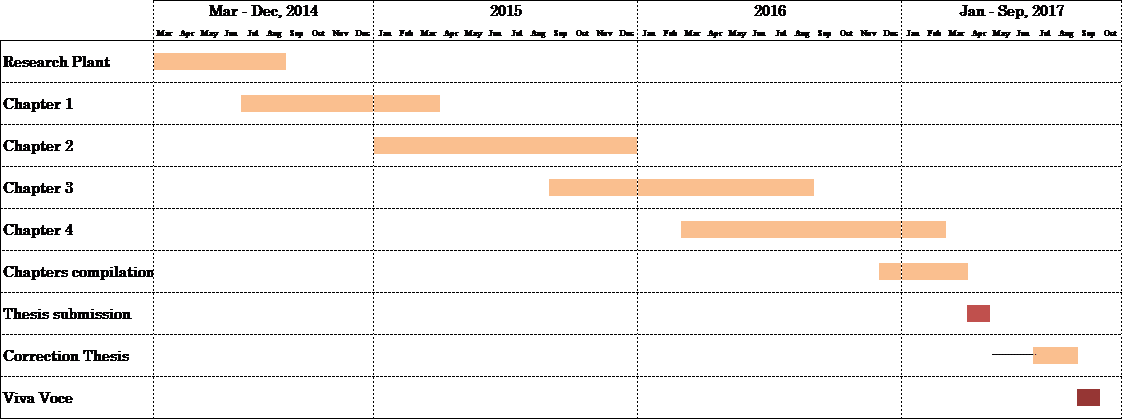
\includegraphics[width=\textwidth]{X11/time-line.png}
   %\captionof{figure}{Caption}
\end{minipage}}
\vspace{2ex}


\end{mdframed}

%% ---------------------------------------------------------------------------
%% 								SECTION 4 
%% ---------------------------------------------------------------------------
\subsubsection*{SECTION 4 --- INFRASTRUCTURE}
\begin{tabular}{ llll }
4.a What are your current infrastructure needs? Are they being met? \\ If not, please describe what arrangements will be made to meet them. & \multicolumn{3}{r}{ \hspace{3cm} $\boxtimes$ Yes $\;$ $\square$ No} \\
\end{tabular}

\begin{mdframed}[everyline=true,splittopskip=20pt,splitbottomskip=20pt]
%\modulolinenumbers[1]
%\internallinenumbers
\vspace{2ex}
\begin{itemize}
\item[$\circledcirc$] Office accommodation that includes a sole-use desk, lockable filing cabinet,  bookshelf facilities and ergonomically sound chair.
\item[$\circledcirc$] Desktop or portable computer, access to networked printing and technical advice.
\end{itemize}

Both bullet points have been provided by the Australian Antarctic Division (AAD). Also on desk space has been provided in facilities of IMAS Taroona.
\vspace{1ex}
\end{mdframed}

\begin{tabular}{ llll }
4.b Are there additional infrastructure needs you anticipate for future stages of your project? \\ Have these been planned for? Please provide details.  & \multicolumn{3}{r}{ \hspace{-0.9cm} $\boxtimes$ Yes $\;$ $\square$ No} \\
\end{tabular}

\begin{mdframed}[everyline=true,splittopskip=20pt,splitbottomskip=20pt]
%\modulolinenumbers[1]
%\internallinenumbers
\vspace{2ex}
\begin{itemize}
\item[$\circledcirc$] Docking Station +  monitor  
\item[$\circledcirc$] Use of cluster computers, mainframe systems, or high performance computing time.
\end{itemize}

The first bullet will be requested once the Research Plan has completed. These equipment  should enhance the performance on tasks like coding and exploration of images.\\
The second bullet point might be required during second year of candidature. Both AAD and IMAS have facilities to make use of this systems. 
\end{mdframed}

%% ---------------------------------------------------------------------------
%% 								SECTION 5 
%% ---------------------------------------------------------------------------
\subsubsection*{SECTION 5 --- DETAILED BUDGET INFORMATION}
The Research Plan may include a  \ul{detailed budget} appropriate to the research project. This budget should be regarded as indicative, an exercise in financial planning and subject to reasonable annual adjustment in the light of the project’s evolution. The intention would be to ensure project costs are compatible with available funds. \textbf{The budget is not an automatic entitlement to spend an allocated amount regardless of the changing needs of the project}. Research related expenses might cover: fieldwork, laboratory consumables, additional library services, off-site photocopying, thesis preparation or any other expenses that can be substantiated as a legitimate cost.

\begin{mdframed}[everyline=true,splittopskip=20pt,splitbottomskip=20pt]
%\modulolinenumbers[1]
%\internallinenumbers
\vspace{2ex}
The budget requested under this PhD research will be utilized to the financing of attendance at international conferences. The main events identified are:

\begin{itemize}
\item[$\circledcirc$] ICES Annual Science Conference (ASC) 2015, which takes place from 21–25 September 2015, in Copenhagen, Denmark.
\item[$\circledcirc$] 7$^{th}$ World Fisheries Congress (WFC), which takes place from 7-11 November 2016 (proposed dates), in Busan, Korea.
\end{itemize}

The projected budget is as follows:

\begin{tabbing}
\hspace{1cm}\=\hspace{3cm}\=\kill
 ICES Conference \>   \>  \\ 
  \>  Perdiem \> AU 1500 \\
    \>  Airfares \> AU 2000 \\
     7$^{th}$ WFC \>   \>  \\ 
  \>  Perdiem \> AU 1500 \\
    \>  Airfares \> AU 1500 \\
         \textbf{Total} \>   \>  \textbf{AU 6500}$^*$
\end{tabbing}

$^*${\footnotesize Sources have not been identified.}
\vspace{2ex}
\end{mdframed}

%% ---------------------------------------------------------------------------
%% 								SECTION 6 
%% ---------------------------------------------------------------------------
\subsubsection*{SECTION 6 --- ETHICS APPROVAL INFORMATION}
You need to consider if your project has ethics implications. The UTAS Research Ethics Policy, information and forms for both Animal and Human (Social Science and Health and Medical) research projects are available from the following web site: \url{http://www.utas.edu.au/research/integrity-and-ethics}\\
\clearpage
If you and your supervisor are uncertain about whether ethics approval is required, please call Integrity and Ethics on 6226 1832 to inquire about ethics requirements. If you require ethics approval, your supervisor and Head of School will need to complete an ethics application.

\textbf{Note: research that requires ethics approval must not commence until approval has been granted. It is University policy that theses cannot be approved for submission to examiners unless all relevant research ethics approvals have been granted.}

\begin{mdframed}[everyline=true,splittopskip=20pt,splitbottomskip=20pt]
%\modulolinenumbers[1]
%\internallinenumbers
\vspace{3ex}
Will your project require any Ethics Committee approval within your period of study?  For example: does your study involve animal experimentation, experiments involving human participants and/or surveys/interviews? \\
$\square$ Yes $\;$ or $\;$ $\boxtimes$ \textbf{No}

Have you obtained ethics approval? $\square$ Yes, my Ethics Approval Ref is: $\ldots\ldots\ldots$ or $\square$ No.

If you require ethics approval, your supervisor and Head of School will need to complete an ethics application.  

\textbf{Note: Ethics approval(s) and approval reference numbers are a requirement of Confirmation of Progression of Candidature within the first year of candidature.}

It is University policy that theses cannot be approved for submission to examiners unless all relevant research ethics approvals have been granted.

\vspace{3ex}
\end{mdframed}

%% ---------------------------------------------------------------------------
%% 								SECTION 7 
%% ---------------------------------------------------------------------------
\subsubsection*{SECTION 7 --- WORK HEALTH AND SAFETY}
Please describe how you will manage any work health and safety issues that will need to be attended to in relation to this project. For details, please refer to the Work Health \& Safety Policy Policies and Procedures at \url{http://www.admin.utas.edu.au/hr/ohs/pol_proc/index.html}

\begin{mdframed}[everyline=true,splittopskip=20pt,splitbottomskip=20pt]
%\modulolinenumbers[1]
%\internallinenumbers
\vspace{5ex}
Induction to Health and Safety at IMAS and AAD were attended
\vspace{5ex}
\end{mdframed}


%% ---------------------------------------------------------------------------
%% 								SECTION 8 
%% ---------------------------------------------------------------------------
\clearpage
\subsubsection*{SECTION 8 --- SIGNATURES/APPROVALS}

Candidate’s Signature\\
I certify that this plan has been discussed with my Supervisors and Graduate Research Coordinator.  I have kept a copy of this document.

%\begin{TAB}(r,1cm,1cm)[5pt]{|l|l|rl|}{|bt|}% (rows,min,max)[tabcolsep]{columns}{rows}
%Candidate:  &  & Date: & 29/08/2014  \\
% Juan Carlos Quiroz  & $\qquad \qquad \qquad \qquad \qquad \qquad \qquad \qquad \qquad \qquad \qquad \qquad \qquad \qquad  $ &  &   \\
%\end{TAB}
%
%Supervisor/s Signature\\
%I certify that this Research Plan complies with disciplinary norms and established guidelines.  I have viewed and approved this Research Plan.
%
%\begin{TAB}(r,1cm,1cm)[5pt]{|l|l|rl|}{|bt|bt|bt|bt|bt|}% (rows,min,max)[tabcolsep]{columns}{rows}
%Primary Supervisor:  &  & Date: & $\qquad \qquad \quad \; $ \\
% Dr. Klaas Hartman  & $\qquad \qquad \qquad \qquad \qquad \qquad \qquad \qquad \qquad \qquad \qquad \qquad \qquad \quad \;  \; $ &  &   \\
% Co-Supervisor:  &  & Date: &    \\
% Prof. Caleb Gardner  &  &  &   \\
%  Co-Supervisor:  &  & Date: &   \\
% Dr. Dirk Welsford   &  &  &   \\
%  Co-Supervisor:  &  & Date: &   \\
% Dr. Philippe Ziegler  &  &  &   \\
%  Co-Supervisor:  &  & Date: &   \\
% Dr. Paul Burch  &  &  &   \\
%\end{TAB}
%
%Graduate Research Co-ordinator’s Signature\\
%I certify that I have viewed and approved this Research Plan.
%
%\begin{TAB}(r,1cm,1cm)[5pt]{|l|l|rl|}{|bt|}% (rows,min,max)[tabcolsep]{columns}{rows}
%Graduate Research  &  & Date: & $\qquad \qquad \quad \; $  \\
%Co-ordinator:  & $\qquad \qquad \qquad \qquad \qquad \qquad \qquad \qquad \qquad \qquad \qquad \qquad \qquad \qquad  $ &  &   \\
%\end{TAB}

\centering{
\textbf{Note: You may add any other relevant additional comments or information and send with this document.}\\

	Please scan and return the signed Research Plan by email to:\\
   
\href{mailto:my_address@wikibooks.org}{Graduate.Research@utas.edu.au}
}



%% ---------------------------------------------------------------------------
%% 								REFERENCES 
%% ---------------------------------------------------------------------------

\bibliographystyle{apa} 
%\nocite{*}
\bibliography{references}

\end{document}
